\section{Diagramas}
\subsection{Diagramas de Clases (UML)}
Para entender correctamente la relación entre las clases, tanto de las ya dadas en el fichero original como de las creadas posteriormente, se ha realizado un diagrama de clases en formato \emph{UML} para ello se ha empleado el programa StarUML\textsuperscript{\textregistered}.

\begin{figure}[h]
    \centering
    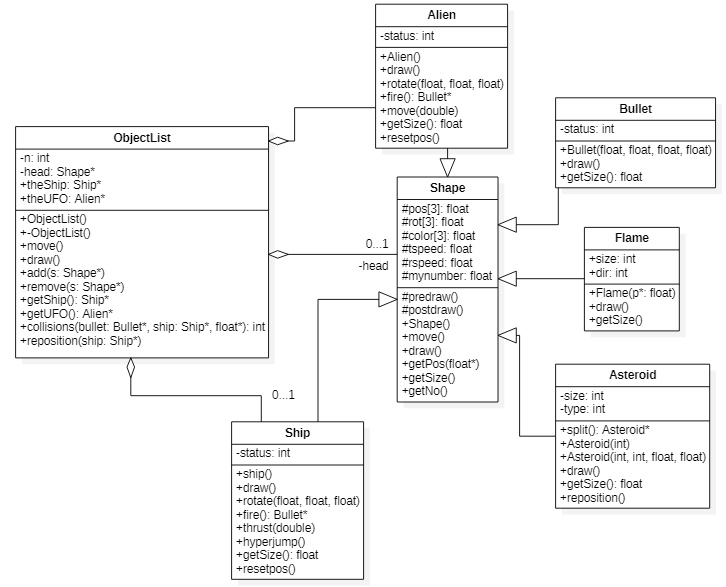
\includegraphics[width=\textwidth]{fotos/UML.PNG}
    \caption{Diagrama de clases del juego mediante \emph{StarUML}}
    \label{uml}
    \end{figure}

Como puede verse en la Ilustración \ref{uml}, la clase \emph{ObjectList} agrega  Al igual que la clase Ship, la clase Alien es hija de la clase Shape y además la clase Alien tiene mucho en común con la clase Ship, pues hace prácticamente lo mismo, con la diferencia de que el OVNI (instancia de la clase Alien) se mueve automáticamente y de forma errática sin ser necesaria la interacción con el usuario. Por comodidad se han añadido dos punteros, uno al OVNI y otro a la astronave, que simplificarán mucho el código tanto en la lógica del juego como en la implementación de la clase ObjectList.
A parte de las clases aquí representadas, existe otro archivo de cabecera llamado commonstuff, que como su nombre indica, almacena funciones cortas, parámetros y llamadas a librerías usadas en todos los archivos fuente del programa.
\subsection{Diagramas de comunicación}


